\documentclass[a4paper,12pt,titlepage]{scrartcl}
\usepackage{graphicx}
\usepackage{url}

\titlehead{
	\centering
	
\includegraphics[width=5in]{images/d3b.png}
	
\includegraphics[width=5in]{images/kidsfirst.png}
}
\title{Developer Handbook}
\date{\today}

\begin{document}

	\maketitle
	
	\tableofcontents
	\newpage
   
	\section{Welcome}
   
	\section{Creating Issues}
	
	Issues should be created 
	If a repository has an {\em Issue Template}, make sure to follow it!
      
	\section{Finding Issues}
	
	\subsection{Labels}
	
	Repositories across the D3b Github organization that have frequent user feedback and bug reports should use our standard set of labels to tag issues shown in Figure \ref{fig:labels}.
	Labels act as a means of filtering categories of issues and providing summaries of effort completed in release notes.
	Users that are not part of the organization may not add labels themselves, so please add labels as you see necessary to new issues.
	The {\b help wanted} label is a special label that is displayed in repository summaries on Github (See the {\em 11 Issues need help} in Figure \ref{fig:reposummary}).
	Use it to mark issues that are self-contained and do not require in-depth knowledge of how the code base works.
	This tag is useful for guiding new members or external contributors looking to get involved to issues that will be easy for them to accomplish.
   
    \begin{figure}
    		\centering
    		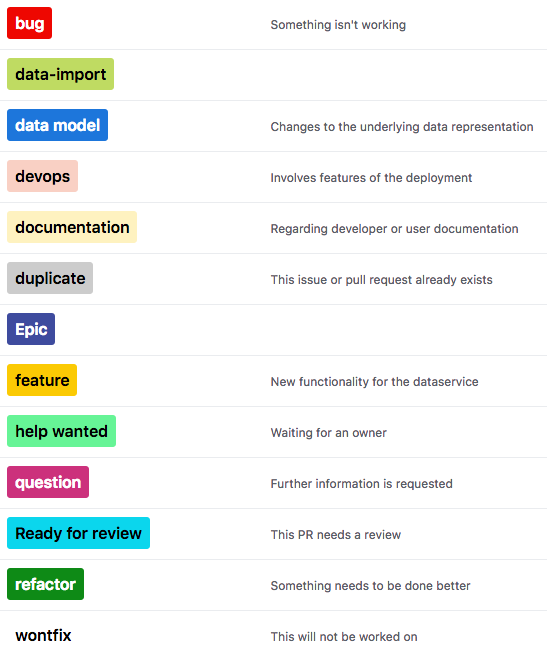
\includegraphics[width=0.6\linewidth]{images/labels.png}
    		\label{fig:labels}
    		\caption{Standard Repository labels with descriptions and colors}
    \end{figure}
	
   
	\section{Creating a Pull Request}
	
	\subsection{Commit Messages}
	
	\subsection{Pull Request Titles}
	
	\subsection{Keeping the Commit Log Tidy}
	
	\subsection{Labeling Pull Requests}
	
	\subsection{Requesting Reviews}
   
	\section{Review Process}
	
	\subsection{Code Review}
	
	\subsection{Testing}
	
	\subsection{Status Checks}
   
	\section{Software Release}
	
	\section{New Repositories}
	
	\subsection{Naming}
	
	\subsection{Description}
	
	\subsection{Tags}
	
	\subsection{Protected Branches}
	
	\subsection{README}
	
	\subsection{License}
	
	Kids First uses the Apache 2.0 \cite{apache2} license exclusively for all public repositories.
	The file should be placed in the root of the directory with the name {\em LICENSE}.
	The Apache 2.0 license may be easily added from the root repository view on Github using {\em add new file} and naming it LICENSE.
	This will present a {\em Choose license template} button to the right of the file name where the Apache 2.0 License may be chosen to automatically populate the file (See Fig \ref{fig:addlicense}).
	
	\begin{figure}
    		\centering
    		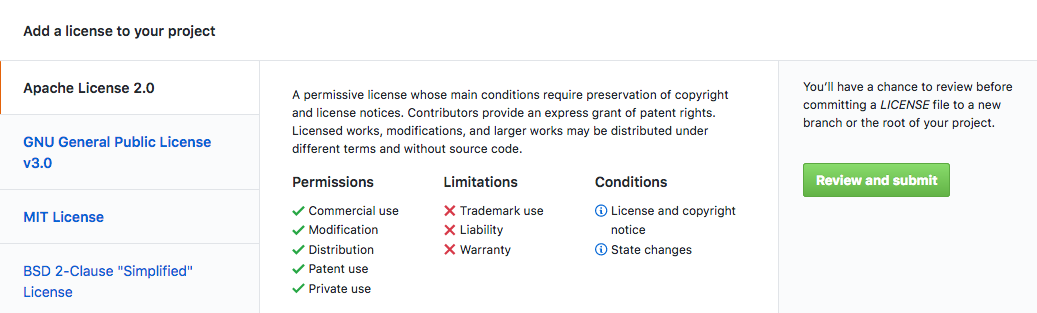
\includegraphics[width=0.8\linewidth]{images/license.png}
    		\label{fig:addlicense}
    		\caption{The Apache 2.0 license is available by default from the Github web interface.}
    \end{figure}
	
	\subsection{Config Repository}
	
	In addition to creating the main code repository, each code repository that is to be deployed must have a second, {\em private} repository that contains the infrastructure and CI/CD strategy for that code base.
	The repository for the config {\em must match the name of the code repository suffixed with -config}.
	This is a rule of thumb that is followed throughout so that the configuration may be discovered automatically by other scripts.
	In addition to the naming standard, the repository should be {\em private}.
	It is best practice to keep the infrastructure obscured and prevent external contributions as the config contains code that is often run at elevated privileges in our environments.
	
	\section{Environments}
	
	Often, entire software stacks are deployed concurrently in many different {\em environments}. This provides us with a handful of benefits:
	
	\begin{itemize}  
	\item Assurance that there is always a stable deployment for end-users
	\item Provides a safe sandbox to develop new features in isolation
	\item Insures the boilerplate to re-deploy a new environment exists
	\end{itemize}
	
	We divide our environments into three primary stages that are tightly couple to our Continuous Integration
	
	\subsection{dev}
	
	The development environment (dev) is intended as sandbox for  new features and code bases.
	It is the most unstable environment with no guarantees on data availability.
	When new code is pushed to a feature branch, it automatically triggers its CI pipeline to test, build, and, deploy to the development environment.
	The branch must pass through testing and deployment successfully to before it is allowed to be merged to insure that it will successfully deploy to the next stage.
	
	\subsection{qa}
	
	The QA environment provides a mostly-stable environment where new features may be used, evaluated, and tested before being released.
	This is is where integration test-suites may be run to ensure that all services cooperate nicely.
	The data in QA should also be close to production quality to fully flex all features.
	New features enter QA after merging a feature branch into the master branch of a code base.
	
	\subsection{prd}
	
	The production environment (prd) is the end-user environment.
	This is critically stable as it must be exposed to the public.
	To introduce features into prd, a repository must go through the release process.
	This includes creating a pull request for the version change, signoff on it from any potential stakeholders, merging, and finally acquiring final approval from an administrator to deploy the infrastructure and code into the environment.
	
	\begin{figure}
    		\centering
    		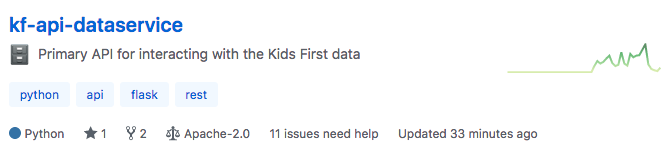
\includegraphics[width=0.6\linewidth]{images/reposummary.png}
    		\label{fig:reposummary}
    		\caption{An exemplary repository summary including: proper naming scheme, emoji followed by short description, labels, the {\em Apache 2.0} license, and issues tagged with {\em help wanted}}
    \end{figure}

	\bibliographystyle{plain}
	\bibliography{bibliography} 
\end{document}